\chapter{Software}

\section{GitLab installation}

\subsection{Data and configuration}

GitLab is installed and running with Docker as container runtime.
All data and configuration files are stored in the home directory ('/home/debian/gitlab') of the debian user on the 'gitlab-ce' machine.

\begin{figure}[H]
	\centering
	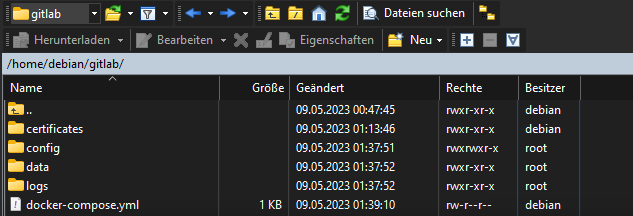
\includegraphics[width=14cm]{images/gitlab_contents.png}
	\caption{GitLab data and configuration}
	\label{fig:gitlab_contents}
\end{figure}

The base configuration for the GitLab Docker image is stored inside the 'docker-compose.yml' file \ref{code:gitlab-compose}.

\lstinputlisting[language=docker-compose-2,caption={GitLab docker-compose.yml},breaklines=false,label={code:gitlab-compose}]{source/docker-compose.yml}

\subsection{Management}

To manage the GitLab instance only 'docker compose' commands are required \ref{code:gitlab-manage}.
\begin{lstlisting}[language=bash,caption={Manage GitLab},label={code:gitlab-manage}]
# start GitLab
/home/debian/gitlab && docker compose up -d
# stop GitLab
/home/debian/gitlab && docker compose down
\end{lstlisting}

\section{GitLab Runner installation}

\subsection{Setup}

In GitLab in the Admin area select 'Runners' and then 'Register an instance runner'.
Follow the description on how to download and install everything fitting to the OS of the Runner (in our case Linux).
Then run the shown command to register the Runner, like shown in \ref{fig:gitlab_add_runner}.

\begin{figure}[H]
	\centering
	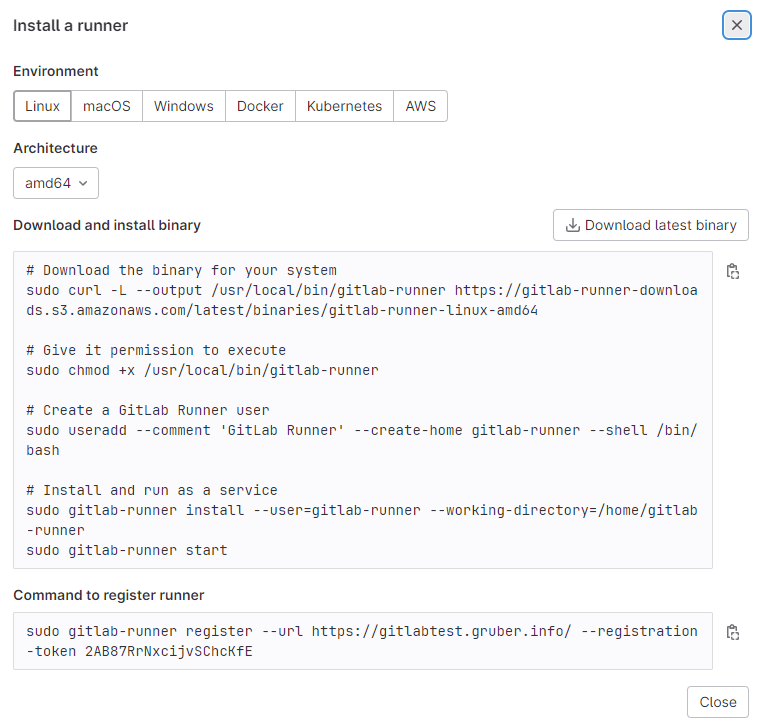
\includegraphics[height=10cm]{images/gitlab_add_runner.png}
	\caption{Add GitLab Runner}
	\label{fig:gitlab_add_runner}
\end{figure}

Afterwards the Runner will be listed in the Runners overview, as shown in \ref{fig:gitlab_list_runners}.

\begin{figure}[H]
	\centering
	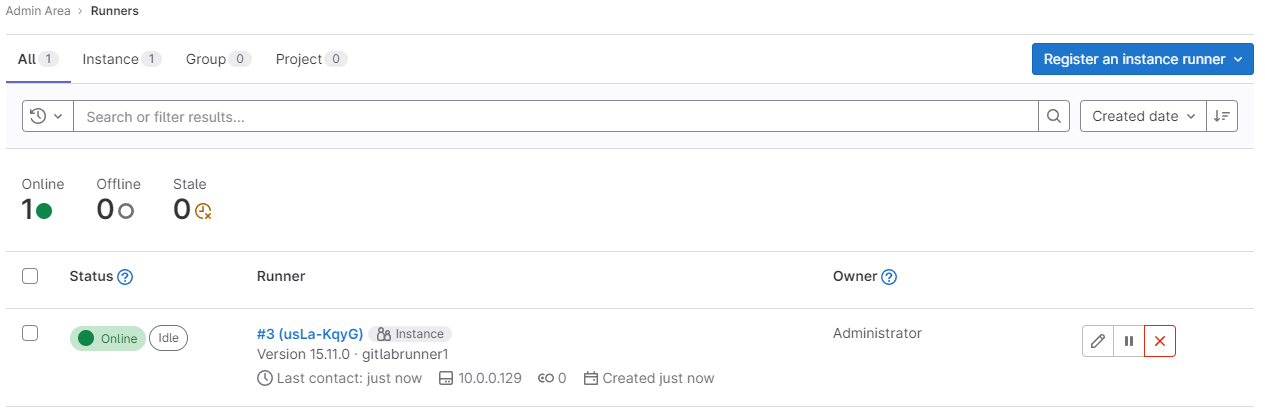
\includegraphics[width=14cm]{images/gitlab_list_runners.png}
	\caption{List of GitLab Runners}
	\label{fig:gitlab_list_runners}
\end{figure}

\subsection{Additional configuration}

The GitLab Runners do their builds in containers.
The container runtime does not respect the '/etc/hosts' file from the host, so within the container 'gitlabtest.gruber.info' always resolves to the public IP.
This causes 'git clone' from our GitLab server to fail from within containers if internet is not available.
Problem and solution is also described on Stackoverflow \cite{refGitlabRunnerHostsFile}.

GitLab Runners provide a configuration option inside their config file ('/etc/gitlab-runner/config.toml'), so it is required to add the host entry from '/etc/hosts' also there, like in \ref{fig:gitlab_runner_extra_hosts}.


\begin{figure}[H]
	\centering
	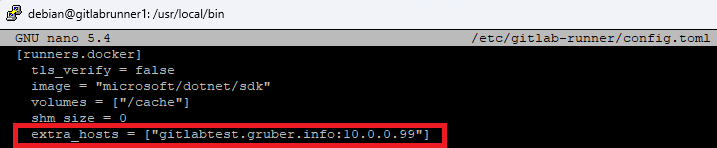
\includegraphics[width=14cm]{images/gitlab_runner_extra_hosts.png}
	\caption{Add extra hosts to GitLab Runners}
	\label{fig:gitlab_runner_extra_hosts}
\end{figure}
